% statistics_and_probability:x02 GDC:NO
\begin{question}
  \hspace*{\fill} [Note maximale: 14]\par
  \noindent Pablo se rend au travail en voiture.\par
  \noindent La probabilité qu’il quitte la maison avant 07 h 00 est de $\frac{3}{4}$.\par
  \noindent S'il quitte la maison avant 07 h 00, la probabilité qu’il soit en retard au travail est de $\frac{1}{8}$.\par 
  \noindent S'il quitte la maison à 07 h 00 ou après, la probabilité qu’il soit en retard au travail est de $\frac{5}{8}$.\par
  \medskip
  (a) Recopiez et complétez le diagramme en arbre suivant.\hspace*{\fill} [3]\par

  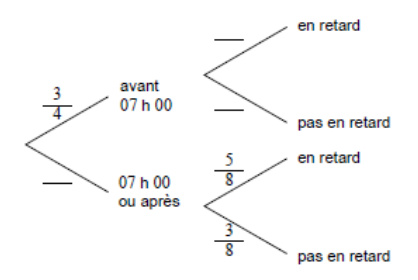
\includegraphics[scale=0.5]{q1_diagram}  

  (b) Trouvez la probabilité que Pablo quitte la maison avant 07 h 00 et qu'il soit en retard.\hspace*{\fill} [2]\par

  (c) Trouvez la probabilité que Pablo soit en retard au travail.\hspace*{\fill} [3]\par

  (d) Sachant que Pablo est en retard au travail,\par
  \hspace{1em}trouvez la probabilité qu’il ait quitté la maison avant 07 h 00.\hspace*{\fill} [3]\par

  (e) Au cours de la semaine prochaine, Pablo se rendra en voiture au travail deux jours.\par
  \hspace{1em}Trouvez la probabilité qu’il soit au moins une fois en retard.\hspace*{\fill} [3]
  
\end{question}

